\documentclass{article}
%\usepackage{fullpage}

\usepackage[english,french]{babel}
\usepackage[utf8]{inputenc}
\usepackage[T1]{fontenc}

\usepackage{amsmath, amsfonts, amssymb, amsthm}
\usepackage{bbm,algorithmic,algorithm,verbatim}
\usepackage[backend=biber,citetracker=true]{biblatex}
\usepackage{color}
\usepackage{subcaption}
\usepackage[pdftex]{graphicx}
\usepackage{epsfig}
\usepackage{ulem, stmaryrd, dsfont}
\usepackage{tikz}
\usepackage{csquotes}
 \usepackage{enumitem}
 \usepackage{float}

% \usepackage{mathabx} % for \vvvert ||| |||
\usepackage{scribe}
\begin{document}
\begin{titlepage}

\newcommand{\HRule}{\rule{\linewidth}{0.5mm}} % Defines a new command for the horizontal lines, change thickness here


%----------------------------------------------------------------------------------------
%	LOGO SECTION
%----------------------------------------------------------------------------------------



\begin{center} % Center remainder of the page

%----------------------------------------------------------------------------------------
%	HEADING SECTIONS
%----------------------------------------------------------------------------------------


\includegraphics[width = 10cm]{index.png}\\[1.5cm] 
\textbf{\textsc{\Large HMMA307: Modeles lineaires avances}}\\[1.0cm] 
\textsc{\Large Université de Montpellier}\\[0.5cm] 
\textsc{\large }\\[0.95cm] 

%----------------------------------------------------------------------------------------
%	TITLE SECTION
%----------------------------------------------------------------------------------------

\HRule \\[0.4cm]
{\huge \bfseries \ Projet HMMA307: Modèles de Régression}\\ % Title of your document
\HRule \\[1.5cm]


%----------------------------------------------------------------------------------------
%	AUTHOR SECTION
%----------------------------------------------------------------------------------------

%\begin{minipage}{0.4\hsize}
\begin{flushleft} \large
\textit{}\\
\vspace{3cm}
\reportauthorOne~Etudiante: Selena Iskounen\\ % Your name
\reportauthorTwo~Enseignant: Joseph Salmon  % Your name
\end{flushleft}

\makeatletter


\end{flushleft}
\vspace{4cm}
\makeatletter


\vfill % Fill the rest of the page with whitespace



\makeatother


\end{titlepage}

\tableofcontents
\newpage
%%%%%%%%%%%%%%%%%%%%%%%%%%%%%%%%%%%%%%%%%%%%%%%%%%%%%%%%%%%%%%%%%%%%%%%%%%%%%%%
%%%%%%%%%%%%%%%%%%%%%%%%%%%%%%%%%%%%%%%%%%%%%%%%%%%%%%%%%%%%%%%%%%%%%%%%%%%%%%%
\section{Introduction}
\label{sec:introduction}

Dans le cadre du cours HMMA307, nous avons étudié le côté théorique de différents modèles visant principalement à la prédiction de variables d'intérêts quelles soit qualitatives ou quantitatives.
Dans ce projet on se propose d'étudier trois modèles particuliers:

\begin{enumerate}
    \item Modèle linéaire mixte avec effet aléatoire
    \item Modèle de régression linéaire
    \item Causalité au sens de Granger
\end{enumerate}
 

Dans un premier temps nous aimerions comparer les résultats obtenus par les deux modèles de régression et comprendre pourquoi le modèle linéaire mixte ne fait pas mieux que le modèle de régression linéaire. Le jeu de données sur lequel nous allons appliquer ces méthodes est le jeu de données $aids$ contenu dans le package $joineR$ du logiciel $R$.\\

Nous allons ensuite appliquer le modèle de régression linéaire sur les données $BostonHousing$ présent sur python sous le nom de $boston$ pour comparer les effets de certaines variables explicatives sur deux groupes. La comparaison de ces deux groupes est basée sur un test d'hypothèses linéaire. 

Pour finir, nous appliquerons un test de Granger sur les données $ChickEgg$ pour savoir s'il y a un effet de causalité entre le nombre d'oeufs et le nombre de poulets, i.e: si le nombre d'oeufs engendrent le nombre de poulets (ou inversement).



L'étude que nous allons effectuer tout au long de ce projet est disponible sur le lien suivant: https://boostedml.com/2019/09/linear-mixed-models-making-predictions-and-evaluating-accuracy.html.


Le jeu de données sur lequel nous allons appliquer ces méthodes est le jeu de données $aids$ contenu dans le package $joineR$ du logiciel $R$.

\vspace{0.5cm}

N.B: On procède comme suit pour charger les dataset sur python: 
\begin{itemize}
    \item On exporte le dataset du logiciel $R$ vers notre ordinateur en utilisant la commande $write.csv$
    \item On importe les données sur python via la commande $pd.read_csv$
\end{itemize}

\newpage
%%%%%%%%%%%%%%%%%%%%%%%%%%%%%%%%%%%%%%%%%%%%%%%%%%%%%%%%%%%%%%%%%%%%%%%%%%%%%%%
%%%%%%%%%%%%%%%%%%%%%%%%%%%%%%%%%%%%%%%%%%%%%%%%%%%%%%%%%%%%%%%%%%%%%%%%%%%%%%%


%%%%%%%%%%%%%%%%%%%%%%%%%%%%%%%%%%%%%%%%%%%%%%%%%%%%%%%%%%%%%%%%%%%%%%%%%%%%%%%
\section{Comparaison du modèle linéaire mixte et le modèle linéaire classique}
%%%%%%%%%%%%%%%%%%%%%%%%%%%%%%%%%%%%%%%%%%%%%%%%%%%%%%%%%%%%%%%%%%%%%%%%%%%%%%%
\subsection{Présentation des données:}
Le tableau de données $aids$ contient un ensemble de données de mesures du nombre de CD4 (globules blancs) ainsi que plusieurs variables qualitatives et quantitatives. Parmis les quantitatives, on retrouve $id$: identité du patient, $time$: temps de mort ou de censure, $death$: décès pendant l'étude, $obtime$: nombre de mois à partir de la première observation. Les variables qualitatives sont: $drug$: type de traitement, $sexe$: femme/homme, $prevOI$: infection antérieur ou pas, $AZT$: intolérance ou echec à l'AZT (zidovudine). Les données sont résumées dans le tableaux suivants:

\begin{figure}[htbp]
    \centering
    \includegraphics{données sida.PNG}
    \caption{Données du tableau $aids$}
    \label{fig:my_label}
\end{figure}

 
%%%%%%%%%%%%%%%%%%%%%%%%%%%%%%%%%%%%%%%%%%%%%%%%%%%%%%%%%%%%%%%%%%%%%%%%%%%%%%%
%%%%%%%%%%%%%%%%%%%%%%%%%%%%%%%%%%%%%%%%%%%%%%%%%%%%%%%%%%%%%%%%%%%%%%%%%%%%%%%
\subsection{Modèle linéaire mixte}
\label{sec:pour_aller_plus_loin_sur_ce_theme}
%%%%%%%%%%%%%%%%%%%%%%%%%%%%%%%%%%%%%%%%%%%%%%%%%%%%%%%%%%%%%%%%%%%%%%%%%%%%%%%
%%%%%%%%%%%%%%%%%%%%%%%%%%%%%%%%%%%%%%%%%%%%%%%%%%%%%%%%%%%%%%%%%%%%%%%%%%%%%%%
\subsubsection{Approche théorique du modèle:}
\subsubsubsection{Equation mathématique du modèle:}

Supposons que nous avons $i = 1,2,........,n$ participants à une étude et pour chaque participant nous avons $j=1,.....,m_i$  observations. 
Soit $y_{ij}$ la mesure de santé du patient $i$ à l'observation $j$. Dans notre cas l'observation $j$ représente la variable $CD4$.

L'équation du modèle linéaire mixte pour notre étude est donc:

\[y_{ij} = \beta_0 + \beta_1 \times x_{ij} + \beta_2 \times z_{ij} +\beat_3 \times u_{ij} + \beta_4 \times s_{ij} + \beta_5 \times r_{ij} + \alpha_{ij} + \epsilon_{ij}\]

\vspace{0.1cm}
\begin{itemize}
    \item $\beta_o$ représente l'intercepte du modèle
    \item $x_{ij}$ la variable $ostime$
    \item $z_{ij}$  la variable $drug$
    \item $u_{ij}$ la variable $gender$
    \item $s_{ij}$ la variable $prevOI$
    \item $r_{ij}$ la variable $AZT$
    \item $\alpha_{ij}$ l'effet aléatoire.
    \item $\epsilon_{ij}$ les résidus.
\end{itemize}

Nous supposons de plus que:
\begin{itemize}
    \item $\epsilon_i \sim \mathcall{N}(0,\Sigma_i)$
    \item $\alpha_{ij} \sim \mathcall{N}(0,G)$ 
    \item le vecteur des résidus $\esplion_{i}$ et l'effet aléatoire $\alpha_{ij}$ sont indépendants.
\end{itemize}


\vspace{1cm}
$Remarque:$

\vspace{0.1cm}
Les effets fixes ($obstime$, $drug$, $gender$, $prevOI$, $AZT$) peuvent être considérés comme des effets moyens sur les patients tandis que l'effet aléatoire $\alpha_{ij}$ est un effet spécifique au patient.

\subsubsubsection;{Estimation du vecteur $\beta_k$:}

Une manière de réecrire l'equation précédente est d'utiliser sa forme matricielle:

\[Y = X \beta  + \epsilon ^*\]

Avec $\epsilon^* =  Z\alpha + \epsilon$\\
D'après l'énnoncé précédent, dans ce cas: $\epsilon^* \sim \mathcall{N}(0,ZGZ^T + \Sigma)$

\vspace{0.1cm}
Posons $V = ZGZ^T + \Sigma $, alors l'estimateur $GLS$ de $\beta$ s'écrit:

\[\beta = (X^T V^{-1} X)^{-1} X V^{-1}y\]


%%%%%%%%%%%%%%%%%%%%%%%%%%%%%%%%%%%%%%%%%%%%%%%%%%%%%%%%%%%%%%%%%%%%%%%%%%%%%%%
%%%%%%%%%%%%%%%%%%%%%%%%%%%%%%%%%%%%%%%%%%%%%%%%%%%%%%%%%%%%%%%%%%%%%%%%%%%%%%%

\subsection{Construction d'intervalles de confiance pour $\hat\beta_j$:}
Supposons que  $Y \sim \mathcall{N} (X \beta, V(\alpha_{ij}))$
et $\hat \beta = X^T V^{-1}(\hat \alpha_{ij} X)^{-1} X^T V^{-1}(\hat \alpha_{ij})$\\
Nous pouvons dériver la matrice de variance covariance de $\hat\beta$ ainsi nous obtenons: \\

\[V(\hat\beta) = (X^T V^{-1}(\hat\alpha_{ij}) X)^{-1}\] \\

Dans ce cas la variance de $\hat \beta$ s'écrit en fonction de la vraie covariance et de la covariance estimée.\\
Lintervalle de confiance de $\hat\beta$ est donné par la formule suivante:\\

\[ [-z_{(1-\alpha)/2} \sqrt{(X^T V^{-1}(\hat\alpha_{ij} X)^{-1}} ;z_{(1-\alpha)/2} \sqrt{(X^T V^{-1}(\hat\alpha_{ij} X)^{-1}] \]


\subsubsection{Application aux données $aids$:}

Les résultats obtenus après application de ce modèle sur les données $aids$ sont résumés dans le tableau suivant:

\begin{center}
    \begin{tabular}{|c|c|c|c|c|}
    \hline
         & Coef & Std.Err & z & P>|z|   \\
         \hline \hline
        Intercept & 5.499 & 0.710 & 7.742 & 0.000\\
         drug[T.ddI] & 0.448 & 0.380 & 1.180 & 0.238 \\
         gender[T.male] & -0..306 & 0.652 & -0.469 & 0.639\\
         prevOI[T.noAIDS] & 4.66 & 0.478 & 9.663 & 0.000\\
         AZT[T.intolerantce]  & 0.261 & 0.472 & 0.554 & 0.579\\
         Group var &  15.253 & 0.683 &  & \\
         \hline
    \end{tabular}
    \captionof{table}{Sorties obtenues par applications du modèle sur $aids$ \texttt{Python}.} 
\end{center}

La sortie $Scale$ est d'autant plus pertinente à analyser car elle représente la variance des résidus (erreur de prédiction?). Dans ce cas et pour ce modèle cette valeur vaut $3.8418$.\\
La colonne $Coef$ représente les estimations du vecteur $\beta_k$ pour $k=0,...,5$.\\
$Group var$ représente l'effet aléatoire.

%%%%%%%%%%%%%%%%%%%%%%%%%%%%%%%%%%%%%%%%%%%%%%%%%%%%%%%%%%%%%%%%%%%%%%%%%%%%%%%
%%%%%%%%%%%%%%%%%%%%%%%%%%%%%%%%%%%%%%%%%%%%%%%%%%%%%%%%%%%%%%%%%%%%%%%%%%%%%%%
\subsection{Modèle de régression linéaire}

\subsubsection{Approche théorique du modèle:}

\subsubsubsection{Equation mathématique du modèle:}

Reprenons les hypothèses du modèle linéaire mixte et gardons les mêmes notations. Dans le cas de la régression linéaire, nous ne disposons plus d'effet aléatoire. L'équation du modèle devient dans ce cas:

\[y_{ij} = \beta_0 + \beta_1 \times x_{ij} + \beta_2 \times z_{ij} +\beat_3 \times u_{ij} + \beta_4 \times s_{ij} + \beta_5 \times r_{ij} + \epsilon_{ij}\]

L'équation matricielle du modèle est:\\
\[Y = X \beta  + \epsilon\]

\subsubsubsection{Estimation de $\beta$:}
Le vecteur $\beta$ est estimé par moindres carrés, son expression est: 
\[\beta = (X^T X)^{-1} X^T y\]

\subsubsection{Application aux données $aids$:}

Les résultats de l'application de ce modèle aux données $aids$ sont résumés dans le tableau suivant:
\begin{center}
    \begin{tabular}{|c|c|c|c|c|}
    \hline
         & Coef & Std.Err & z & P>|z|   \\
         \hline 
         obstime & -0.0840 & 0.025 & -3.325 & 0.001\\
         ddI & 2.2923 & 0.135 & 16.937 & 0.000 \\
         male & 1.6945 & 0.176 & 9.611 & 0.000\\
         noAIDS &4.2548 & 0.176 & 24.217 & 0.000\\
         intolerantce  & 2.1173 & 0.144 & 14.729 & 0.000\\
        
         \hline
    \end{tabular}
    \captionof{table}{Sorties obtenues par applications du modèle linéaire sur $aids$ \texttt{Python}.} 
\end{center}

Comme précédemment, la colonne $Coef$ représente l'estimateur du vecteur $\beta$.\\
Il est pertinent d'analyser la sortie $R-squared$ qui représente le $R^2$ du modèle, ici $R^2 = 0.204$ , on constate qu'il est relativement faible.



%%%%%%%%%%%%%%%%%%%%%%%%%%%%%%%%%%%%%%%%%%%%%%%%%%%%%%%%%%%%%%%%%%%%%%%%%%%%%%%
%%%%%%%%%%%%%%%%%%%%%%%%%%%%%%%%%%%%%%%%%%%%%%%%%%%%%%%%%%%%%%%%%%%%%%%%%%%%%%%
\subsection{conclusion}
Dans cette partie, nous avons montré que le modèle linéaire mixte ne faisait pas mieux que le modèle linéaire avec un effet aléatoire uniquement.

%%%%%%%%%%%%%%%%%%%%%%%%%%%%%%%%%%%%%%%%%%%%%%%%%%%%%%%%%%%%%%%%%%%%%%%%%%%%%%%
%%%%%%%%%%%%%%%%%%%%%%%%%%%%%%%%%%%%%%%%%%%%%%%%%%%%%%%%%%%%%%%%%%%%%%%%%%%%%%%
\section{Comparaison de deux groupes avec un modèle de régression linéaire}

\subsection{Approche théorique:}
Supposons que l'on dispose de $n$ données que nous scindons en deux groupes notés $A$ et $B$ et des variables explicatives noté $x_i$. Nous souhaitons modéliser $E[y_A|x_i]$ et $E[y_B|x_i]$ pour cela nous allons utiliser un modèle de régression linéaire.\\
La question à laquelle nous souhaitons répondre est: y a t-il une différence entre les groupes en tenant compte de certaines variables? \\
Répondre à cette question revient à tester les hypothèses suivantes:\\

$H_0$: $E[y_A|x_i]$= $E[y_B|x_i]$ VS $H_1$:$E[y_A|x_i]$ $\neq$ $E[y_B|x_i]$

\vspace{0.5cm}

Notons: $I(A) = \left\{
    \begin{array}{ll}
        \ 1  & group A \\
        \ 0  & group B
    \end{array}
\right.$
et 
$I(B) = \left\{
    \begin{array}{ll}
        \ 1  & group B \\
        \ 0  & group A
    \end{array}
\right.$

\vspace{0.5cm}
Le modèle de régression linéaire est dans ce cas donné par:
\[y_{i} = \beta_0 +\beta_{0,A} \times I(A) + \beta_{1,A} \times x_{1,A} \times I(A) + \beta_{1,B} \times x_{1,B} \times I(B) +.....+ \beta_{p,A} \times x_{p,A} \times I(A) + \beta_{p,B} \times x_{p,B} \times I(B) + \epsilon_{i}\]




\subsection{Présentation des données:}

Nous allons travaillé ici avec les données $boston$ de $Python$ qui correspondent à des données de logement récoltées sur 506 secteurs de Boston contenant $13$ variables explicatives quantitatives tel que "RM" qui correspond au nombre de chambre dans l'appartement. La variable à expliquer est la variable $MEDV$ qui correspond au prix du mètre carré de chaque appartement. 

\vspace{0.2cm}

Nous allons appliqué cette partie théorique aux données $boston$ de $Python$ pour comprendre s'il y a une différence d'effet de crimes (variable $CRIM$), taxes (variables $TAX$) et le statut social du propriétaire (variables $LSTAT$) entre les appartements constitués de plus de 6 chambres et les appartement contenant moins de 6 chambres. Nos deux groupes $A$ et $B$ sont alors:

\vspace{0.2cm}
$A$: appartement de plus de $6$ chambres.\\
$B$: appartement de moins de $6$ chambres.

\newpage

Les données sont résumées dans le tableau suivant:
\begin{figure}[htbp]
    \centering
    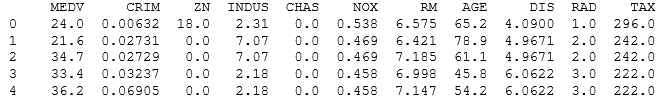
\includegraphics{Capture88.PNG}
    \caption{Données $boston$}
    \label{fig:my_label}
\end{figure}

\subsection{Résultats de la régression linéaire:}
Après avoir scinder les données en deux groupes énoncées précédemment, nous appliquons une régression linéaire sur le groupe $B$ et nous obtenons les résultats résumés dans le tableau suivant:
\begin{center}
    \begin{tabular}{|c|c|c|c|c|}
    \hline
         & Coef goupe B & Coef groupe A    \\
         \hline 
         Intercept  & 37.5979 & 25.5981 \\
         CRIM  & -0.02872 & -0.1209\\
         TAX B & 0.000102 & -0.000255 \\
         LSTAT B & -1.2238   & -0.3719\\
         
         \hline
    \end{tabular}
    \captionof{table}{Sorties obtenues par applications du modèle linéaire sur les données $boston$ du groupe $B$ et $A$ \texttt{Python}.} 
\end{center} 


\subsection{Conclusion:}

L'interprétation des coefficients obtenus précédemment peut se faire de la manière suivante:
\begin{itemize}
    \item Les crimes un léger effet sur le prix des appartements du groupe $B$.
    \item Les taxes ont le même effet pour les appartements du groupe $A$ et ceux du groupe $B$
    \item Le statut social du propriétaire à quant à lui un effet significatif sur le prix des appartements du groupe $B$.
\end{itemize}

%%%%%%%%%%%%%%%%%%%%%%%%%%%%%%%%%%%%%%%%%%%%%%%%%%%%%%%%%%%%%%%%%%%%%%%%%%%%%%%
\section{La causalité au sens de Granger}
%%%%%%%%%%%%%%%%%%%%%%%%%%%%%%%%%%%%%%%%%%%%%%%%%%%%%%%%%%%%%%%%%%%%%%%%%%%%%%%
\subsection{Approche mathématique:}
Supposons que nous avons deux séries chronologiques x et y. La question qu'il serait légitime de poser est: si on observe des décalages sur la série x avec laquelle on prédit y, est-ce que ces derniers controlent les décalages de la série y? \\
Il s'agit ,en mathématiques, du test de Granger univarié.

Une façon de tester cela serait de commencer par définir un modèle linéaire:
\[y_n = \beta_0 x_n + \beta_1 x_{n-1} + \beta_2 x_{n-2} + \beta_k x_{n-k} + \beta_{k+1} y_{n-1} + \beta_{2k} y_{n-k} + \epsilon_n\]

Les hypothèses que l'on teste sont les suivantes:

$H_0$ : $\beta_1 = \beta_2 = ... = \beta_k$ les décalages de $x$ n'engendre pas de décalages de $y$.

$H_1$ : $\exists$  $i \in [1,k]$ tq $\beta_i = 0 $ les décalages de $x$ engendrent des décalages de $y$.

\subsection{Présentation des données:}
Dans cette partie, on se propose d'appliquer un test de Granger aux données $chicken$ constituées de deux colonnes: La première représente le nombre de poulets  et la seconde le nombre d'oeufs produit par ces poulets aux USA de 1930 à 1983.

\begin{figure}[htbp]
    \centering
    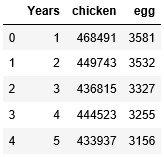
\includegraphics{chicken.PNG}
    \caption{Données $chicken$}
    \label{fig:my_label}
\end{figure}

\subsection{Application aux données $chicken$:}

 On cherche à tester: $H_o$: les décalages du nombre d'oeufs n'engendrent pas des décalages sur le nombre de poulets, VS $H_1:$ les décalages du nombre d'oeufs engendrent des décalages sur le nombre de poulets.\\
 Dans un premier temps, nous allons nous intéresser à la courbe des deux séries chronologiques.

\begin{figure}[htbp]
    \centering
    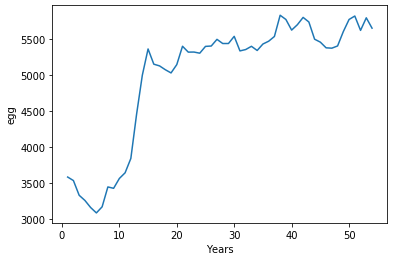
\includegraphics{oeuf.PNG}
    \caption{Variation du nombre d'oeufs de 1930 à 1983}
    \label{fig:my_label}
\end{figure}

\begin{figure}[htbp]
    \centering
    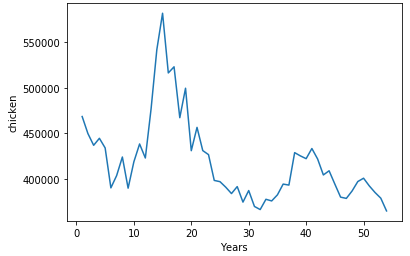
\includegraphics{poulet.PNG}
    \caption{Variation du nombre de poulet de 1930 à 1983}
    \label{fig:my_label}
\end{figure}

$Remarque:$

\vspace{0.1cm}
L'axe des années sur les graphes précédant se lit comme suit: $0$ correspond à $1930$, $10$ correspond à $1940$.... et $50$ correspond à $1980$.

\vspace{0.2cm}
Nous remarquons que le nombre de poulet varie significativement entre $1930$ et $1950$ tandis que le nombre d'oeufs est essentiellement croissant. Il serait donc légitime de penser que le nombre de poulets n'influe pas sur le nombre d'oeufs.

\subsection{Résultats du test de Granger:}

Les résultats obtenus après application de la causalité au sens de Granger sur les variables $chicken$ et sur les $egg$ sont résumés dans le tableau suivant:
\begin{center}
    \begin{tabular}{|c|c|c|c|c|}
    \hline
         & Chicken B & Egg    \\
         \hline 
         F  & 5.4050 & 0.5916 \\
         p-value  & 0.003 & 0.06238\\
         df_denom & 44 & 44 \\
         df_num & 3  & 3\\
         
         \hline
    \end{tabular}
    \captionof{table}{Sorties obtenues par applications du test de Granger sur les données $chicken$ \texttt{Python}.} 
\end{center} 

Nous remarquons que la p-value obtenue pour le test de Granger concernant $chicken$ est inférieur à $0.05$ , nous serions donc tenter d'affirmer que le nombre d'oeufs influe significativement sur le nombre de futur poulet. Pour s'en assurer nous faisons le test dans l'autre direction, cette fois ci la p-value est supérieur à $0.05$. Le nombre de poulets n'influe pas sur le nombre d'oeufs.

\subsection{Conclusion:}

Nous ne pouvons pas affirmer qu'il y ait un effet de causalité entre le nombre de poulets et le nombre d'oeufs.
\end{document}